\section{Introduction}
\label{sec:intro}

\epigraph{
    ``Well, my dear, convenience might mean something completely different to a Japanese user vs. an American user.''
}{
    Phoebe Yu~\cite{Yu2024}
}

Since its inception in 1989, the \ac{www} has made digital knowledge sharing through hyperlinked websites accessible to people worldwide.
Today, this access to information is available to, and further developed by, people from diverse cultural backgrounds.
This chapter provides an overview of the motivation behind this research, defines the research questions, and states the specific objectives of the study.
It also outlines the structure of this thesis.

\subsection{Background and Motivation}
\label{sec:intro-background-and-motivation}

Human cultures have roots in experiences from millennia ago, with cultural values being persistently passed down through generations.
In contrast to these vast timescales, the \ac{www} is a relatively recent development.
It is thus natural to assume that contributions to the \ac{www} are influenced by individual cultural characteristics, despite the globalized nature of the technology.

Two perspectives can be considered in this regard: that of software users and that of software developers.
A multitude of factors, including educational backgrounds and regional coding standards, suggests that the way websites are developed and consumed may vary across different geographic regions.

Understanding these global variations is crucial for any international actor, whether in business or research.
Recognizing and adapting to these differences can, for instance, enhance the user experience of regionally tailored websites, boosting engagement and potentially increasing sales.
Moreover, international companies can improve the efficiency and effectiveness of their web development teams by aligning coding practices with regional strengths.
Additionally, insights into dependencies among web resources can significantly aid supply chain security.

This thesis is motivated by a desire to systematically analyze and understand these global variations in website data.
Here, website data is understood not only as \ac{html}, \ac{css}, and \ac{js} but also as metadata, including timing measurements and information on server locations.
The hypothesis driving this research is that website data exhibits distinct variations based on the geographic location of developers.
The primary aim of this research is to empirically test this hypothesis by designing and implementing a reusable data pipeline that can subsequently be utilized by future researchers to address further questions on large-scale web data.

An illustrative example serves to introduce this thesis: the two websites shown in \cref{fig:hanko} and \cref{fig:fax-machine} display noticeable visual differences in web design.

\begin{figure}[H]
    \centering
    \begin{subfigure}{.45\textwidth}
      \centering
      
\includegraphics[width=\linewidth]{figures/hankoya.png}
      \caption{A specialist retailer's website, aiming for convenience through information density, showcases a historical device still in use for administrative processes in Japan: stamps~\cite{Ha24}.}
      \label{fig:hanko}
    \end{subfigure}
    \hspace{0.025\textwidth}
    \begin{subfigure}{0.45\textwidth}
      \centering
      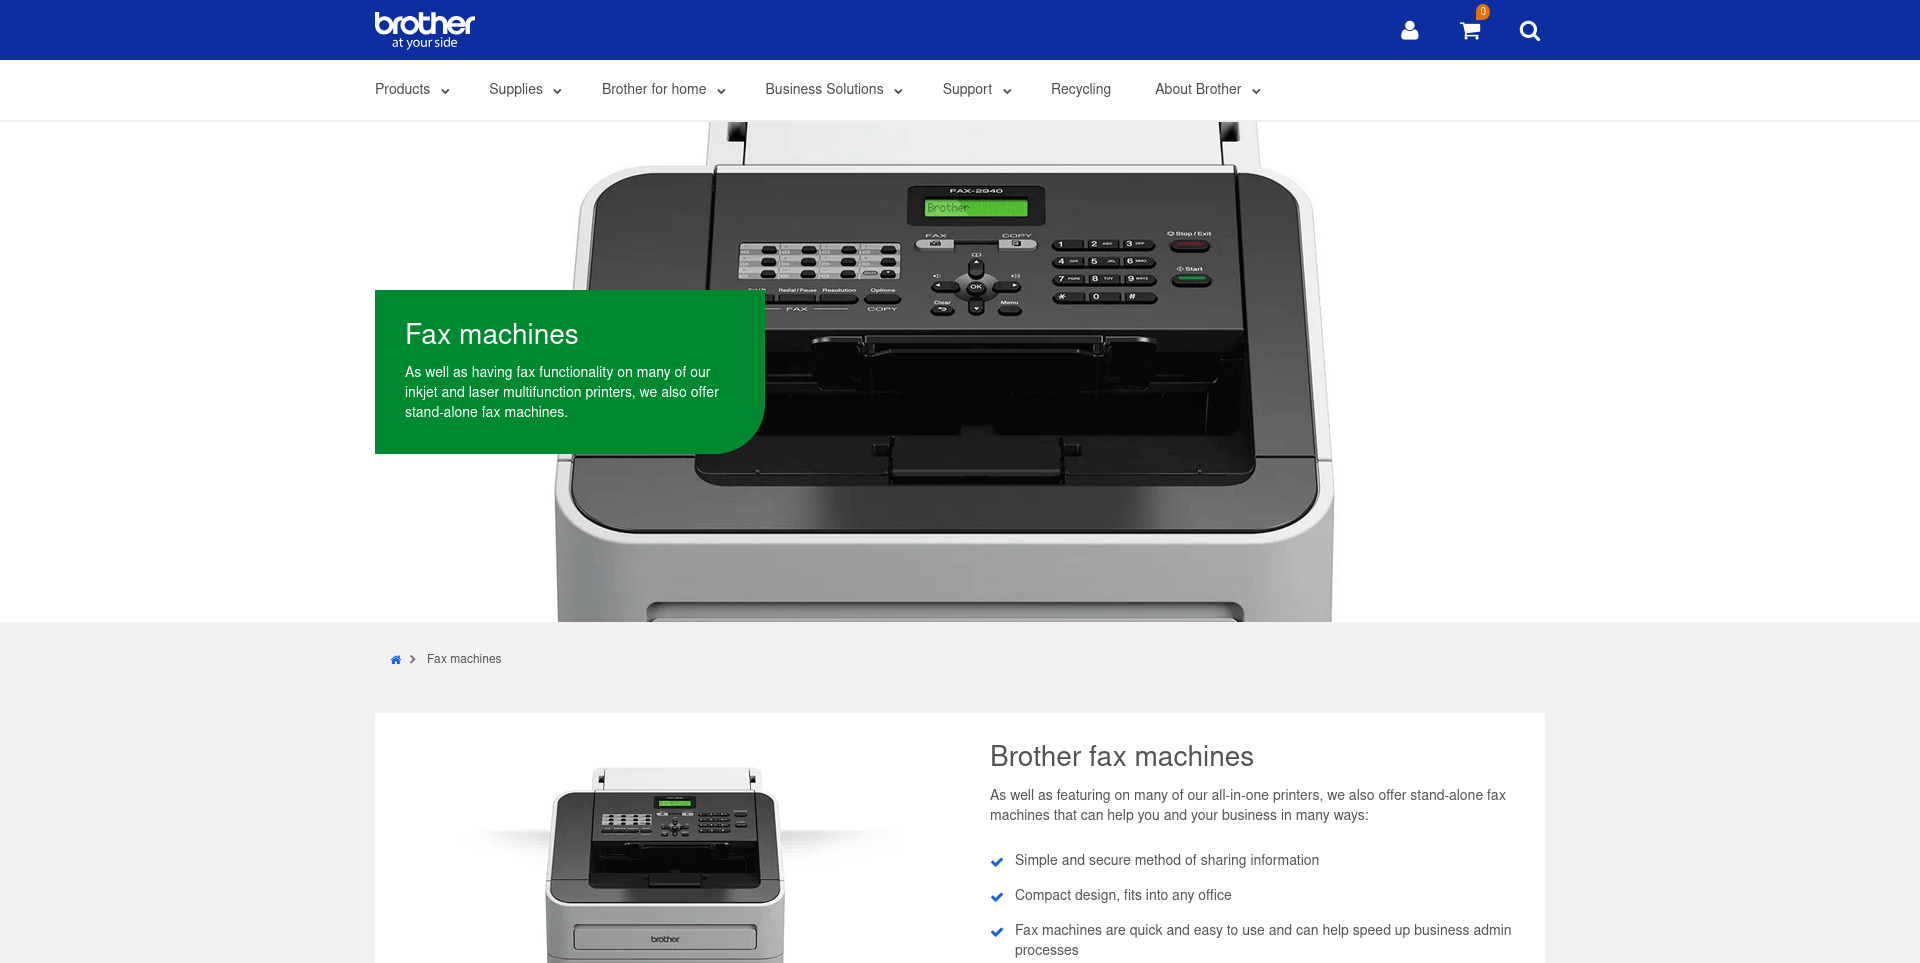
\includegraphics[width=\linewidth]{figures/brother.png}
      \caption{A specialist retailer's website, aiming for convenience through cleanliness, showcases a historical device still in use for administrative processes in Germany: fax machines~\cite{Br24}.}
      \label{fig:fax-machine}
    \end{subfigure}
    \caption{Introductory example for differences in web design.}
    \label{fig:intro-examples}
\end{figure}

While Western websites often use whitespace to create a clean, focused appearance, Japanese culture values high information density on each page as a form of convenience and perceived control.
This observation is reflected in the epigraph preceding this chapter.


\subsection{Research Question}
\label{sec:intro-research-question}

Building on the background provided in the previous section, the primary research question guiding this thesis is:

\begin{enumerate}
    \item[] \Question{rq:0}{Can we test or refute hypotheses on global variations in website code?}

    Our expectation is that such global variations can be detected and analyzed using a Big Data pipeline specifically created for this purpose.
    However, several factors could complicate the results or, in the worst case, make them unattainable.
    These factors include potential issues such as selecting a suboptimal dataset for ingestion, which might contain insufficient meaningful information, challenges in technical implementation, or possible ambiguities in the results.
    Additionally, the variations sought in this research may diminish or even disappear over time as globalized standards, like universal code styles, find worldwide application across projects.

    To address the broad primary research question stated above, the following sub-questions are of implicit interest:

    \item[] \Question{rq:1}{What influence does culture have on code?}

    The motivation for this thesis is rooted in the intuition that human culture influences how code is written.
    This question aims to establish the general context for the study.
    If no cultural influence on code exists, our intuition would be incorrect—an outcome that should always be considered a possibility.
    Such a finding would still allow for the existence of global code variations; these variations would simply not be related to cultural differences, allowing the research to continue even if the initial assumption is disproven.

    \item[] \Question{rq:2}{Which global variations in code have been researched before?}

    This practical question about the scientific context aims to ensure that this thesis provides highest academic benefit by avoiding redundancy with previous efforts.
    Additionally, referencing variations identified in prior research allows for validation checks on our findings through benchmarking comparison.
    Finally, understanding the extent of existing research into this topic helps determine whether further theoretical or practical results would be beneficial to the current scientific community.
    The answer to this question should yield two primary insights, guiding the focus of the following chapters, which are articulated as subquestions below.

    \begin{enumerate}
        \item[] \subQuestion{rq:21}{Which specific feature patterns in website code can be identified and analyzed for global variations?}

        This thesis is intended as foundational work that can support future expansions in global web analysis.
        Although this study primarily focuses on \ac{html}, other aspects of websites should be examined to reach holistic conclusions on global code variations.
        Analysis could range from measuring document sizes to timing web resource connection speeds.
        Defining a scope of feature patterns to analyze clarifies which areas remain open for future research.

        \medskip
        \item[] \subQuestion{rq:22}{Which statistical methods and algorithms are effective in detecting global variations in website code?}

        Assuming the pipeline design successfully processes data as specified by our objectives in \cref{sec:intro-objectives}, an evaluation of the resulting data is necessary to draw meaningful conclusions.
        It is therefore essential to make an informed decision on which evaluation methods or algorithms to use for optimal results.
    \end{enumerate}

    \item[] \Question{rq:3}{Which data sources can be used to yield valuable insights?}

    After clarifying cultural influences on code and previous research, it is necessary to identify data sources that support the research.
    To cater to varying interests among fellow researchers, this question is divided into two sub-questions: one addressing publicly available data and another considering private data sourcing.
    To stay focused on the primary research question, the topic of private data sourcing is discussed in an advisory manner, to avoid potentially confusing diversions from the main topic.

    \begin{enumerate}
        \item[] \subQuestion{rq:31}{Which datasets include the feature patterns under study and are publicly available?}

        Selecting suitable datasets increases the likelihood of producing actionable results.
        Additionally, the answer to this question may clarify the need for flexible ingestion of various data formats, as data archives might store websites in compressed formats rather than in their original state.
        Finally, utilizing publicly available datasets allows for reproducibility of this thesis's findings.

        \medskip
        \item[] \subQuestion{rq:32}{In which ways can useful datasets be sourced independently?}

        One may opt to source data independently to reduce reliance on external data providers or to analyze specific features that are not part of a publicly available dataset.
        While manually fetching features one by one is inefficient, knowledge of automated data-sourcing methods can be an advantageous addition to one's toolkit.
    \end{enumerate}

    \item[] \Question{rq:4}{What is the current state of Big Data and data engineering?}

    This question establishes a foundation for two more detailed questions on modern Big Data pipelines.
    Understanding the evolution of Big Data is essential for contextualizing how data pipelining fits within the broader field of data engineering.

    \begin{enumerate}
        \item[] \subQuestion{rq:41}{What constitutes a modern Big Data pipeline design?}

        Big data analyses are increasingly popular as datasets of substantial size become accessible to the public.
        Google Trends data show that global searches for ``big data'' began to rise around 2011 and peaked in 2017, as shown in \cref{fig:trends-big-data}.
        Similarly, \cref{fig:trends-data-pipeline} illustrates that worldwide searches for ``data pipeline'' increased in 2016 and have since trended upwards.

        \begin{figure}[H]
            \centering
            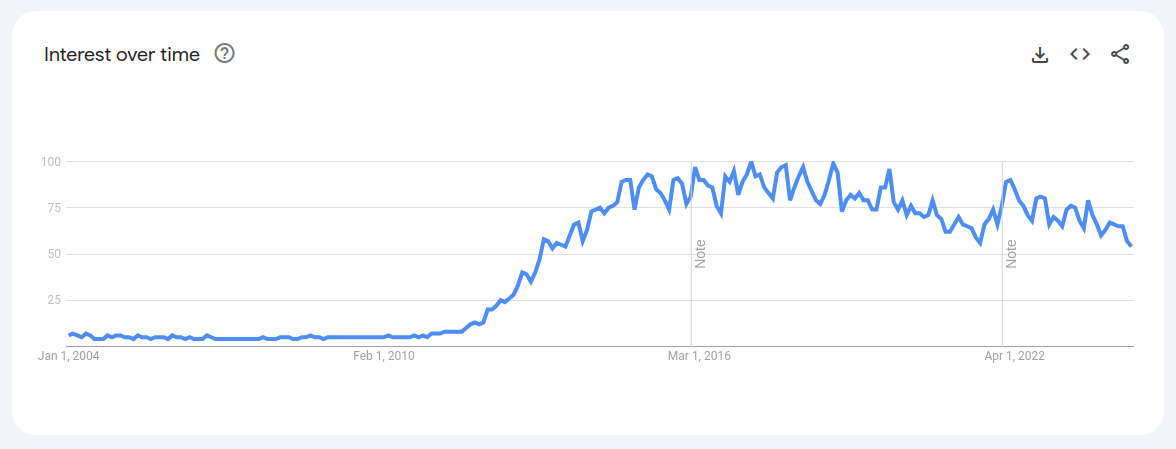
\includegraphics[width=\textwidth]{figures/trends-big-data.png}
            \caption{Google Trends data for worldwide searches of the term ``big data'' from 2004 to the present~\cite{Go2024}.}
            \label{fig:trends-big-data}
        \end{figure}

        \begin{figure}[H]
            \centering
            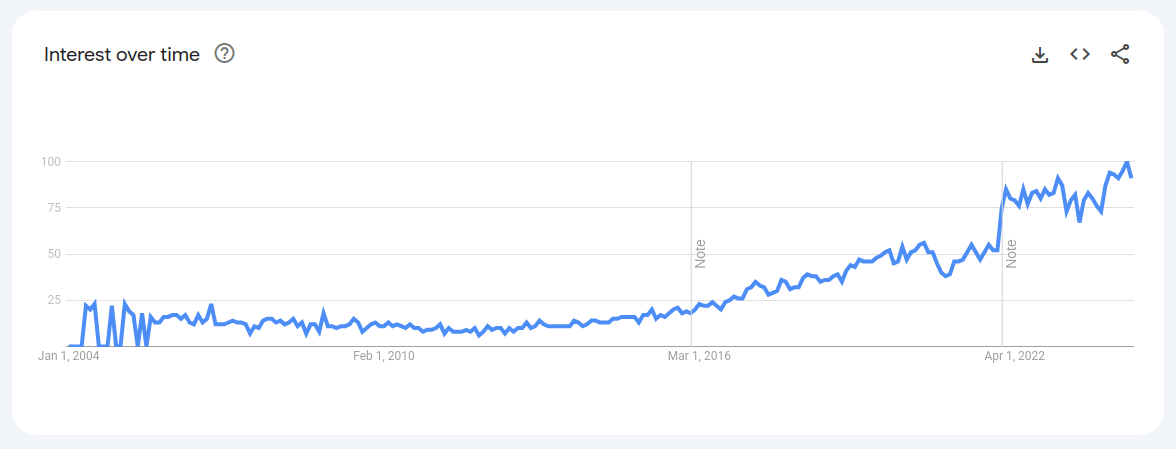
\includegraphics[width=\textwidth]{figures/trends-data-pipeline.png}
            \caption{Google Trends data for worldwide searches of the term ``data pipeline'' from 2004 to the present~\cite{Go2024}.}
            \label{fig:trends-data-pipeline}
        \end{figure}

        From these trends, it can be concluded that Big Data pipeline design remains an area of active development, in which universally agreed-upon standards might not yet exist.
        The pipeline designed in this thesis should prioritize support for the most promising advancements in Big Data pipeline research over commercial usefulness.

        \medskip
        \item[] \subQuestion{rq:42}{How can the effectiveness and accuracy of the pipeline be benchmarked?}

        This question is intended to be addressed only briefly in this thesis, as it represents a potential topic for future in-depth research.
        However, the work in this thesis will establish a foundation for a qualitative evaluation of the findings.
        Through a thorough literature review, methods will be identified to sufficiently validate the pipeline's effectiveness and accuracy, aiming to support a clearer interpretation of the results' significance.
    \end{enumerate}
\end{enumerate}

These questions aim to explore the core hypothesis of this thesis, guiding the design, implementation, and analysis of the proposed data pipeline system.


\subsection{Objectives}
\label{sec:intro-objectives}

Complementary to the theoretical foundation laid out in \cref{sec:intro-background-and-motivation} above, the primary practical aim of this thesis is to develop a scalable data pipeline capable of ingesting, processing, and analyzing website code from around the world.
The pipeline design should adhere to contemporary data engineering methodologies, enabling large volumes of data to flow smoothly.
These are our objectives:

\begin{enumerate}
    \item \textbf{Design and implement a scalable data pipeline}

    The system should be capable of handling diverse data formats and allow for flexible incorporation of additional data sources in the future.
    While \ac{html} is the primary candidate for analysis due to its accessibility, the pipeline should not be restricted to specific data formats or programming languages.
    Instead, it should accommodate any machine-readable data related to websites, including both well-structured sources, such as Common Crawl, and less-structured data, like transmission logs or potentially incomplete data such as the initial bytes of a website's HTML code.
    Additionally, the pipeline design should aim to use storage space as efficiently as possible.
    The pipeline should enable:

    \begin{enumerate}
        \item ingestion of diverse data sources, including both well-structured and less-structured data,
        \item transformation, analysis, and visualization of key metrics to yield insightful results, and
        \item persistence of ingested data and derivatives with minimal compute and storage usage.
    \end{enumerate}

    \item \textbf{Identify and quantify global variations in website code}

    Following the implementation and operation of the system, a visualization tool should be selected and configured to effectively represent the data returned by the pipeline.
    The visualizations provided should assist in interpreting and understanding the analysis results.

    \item \textbf{Evaluate the qualitative performance of the data pipeline}

    Assess the accuracy and reliability of the proposed system in detecting and analyzing global variations in website code, including evaluating the precision of variation detection and the system's ability to handle datasets at scale.
    The central outcome of all data processing, analysis, and evaluation efforts should be the capacity to confidently identify feature patterns that exhibit global variations.

    \item \textbf{Formalize a data ingestion module definition}

    Finally, this thesis will provide guidelines for future research that the pipeline will facilitate.
    These guidelines will enable researchers to incorporate additional data sources, refine analysis techniques, and enhance system performance, thereby contributing to ongoing research in this field.
\end{enumerate}

\subsection{Thesis Structure}
\label{sec:intro-thesis-structure}

This thesis is organized into chapters that progressively build a comprehensive understanding of the research and its findings.
Following the introduction provided in this chapter, the next chapter covers important related work, reviewing existing literature on cultural dimensions, global variations in website code, Big Data, and data engineering.
It establishes the context for the research and identifies the gaps addressed by this thesis.

With a clear scope established, the third chapter outlines the intended system design.
It describes the intuitive approach and details the composition of the data pipeline, including the processes of extracting, loading, and transforming data, as well as visualization strategies.

Chapter four moves on to the implementation phase, detailing the practical steps taken to set up the storage and compute infrastructure, as well as the pipeline's ingestion, transformation, and visualization layers.
It also explains how \ac{dx} is ensured and how the overall system is deployed to production.

The fifth chapter presents the analysis and results.
It showcases several graphs that provide insight into the processed dataset and reports on the pipeline's performance, \ac{dx}, and perceived reliability during operation.

In the sixth chapter, the focus shifts to evaluating the results.
This includes discussions on the implications of the findings, study limitations, potential biases, and the scalability and extensibility of the system.

The seventh chapter explores future work, suggesting directions for further research as well as potential improvements to the system.
Possible extensions, optimizations, and replacements for several parts of the pipeline are suggested to enhance the pipeline's flexibility.

Finally, the eighth chapter concludes this thesis by summarizing its contributions and findings and reflecting on the relevance of the research to the fields of Big Data and web development.
